\documentclass{article}
\usepackage{amsmath}

\usepackage{tikz}
\usepackage{circuitikz}
\usetikzlibrary{shapes,arrows,positioning}

\usepackage{geometry} % Required for customizing margins
\geometry{margin=1in} % Sets 1-inch margins on all sides

\begin{document}

\subsection*{Problem 1:}
Consider the system described by the following ordinary differential equation:
\begin{equation*}
\frac{d^2y(t)}{dt^2} + 5\frac{dy(t)}{dt} + 6y(t) &= \frac{dx(t)}{dt} + 5x(t)
\end{equation*}
where \(x(t)\) is the input and \(y(t)\) is the output.

\subsubsection*{(a) [10 points]}Write down the transfer function of this system.

\subsubsection*{(b) [10 points]}
Plot the block diagram and the signal flow graph of this system.

\subsubsection*{(c) [10 points]}
Is this system stable? Why?

\subsubsection*{(d) [10 points]}
Compute the output \(y(t)\) of the system in response to the unit step input \(x(t) = u(t)\), assuming that \(y(0) = 0\) and \(y'(0) = 0\). (\textit{Hint: \(\mathcal{L}[e^{-at}u(t)] = \frac{1}{s+a}\)})

\newpage

\subsubsection*{(a)}

To find the transfer function, we'll take the Laplace transform of the differential equation. Given:
\begin{equation}
\frac{d^2y(t)}{dt^2} + 5\frac{dy(t)}{dt} + 6y(t) = \frac{dx(t)}{dt} + 5x(t)
\end{equation}
Taking the Laplace transform:
\begin{equation}
s^2Y(s) - sy(0) - y'(0) + 5[sY(s) - y(0)] + 6Y(s) &= sX(s) + 5X(s)
\end{equation}
Using the initial conditions \(y(0) = 0\) and \(y'(0) = 0\):
\begin{equation}
s^2Y(s) + 5sY(s) + 6Y(s) &= sX(s) + 5X(s)
\end{equation}
\begin{equation}
Y(s)(s^2 + 5s + 6) &= X(s)(s + 5)
\end{equation}
Thus, the transfer function \( H(s) \) is:
\begin{equation}
H(s) = \frac{Y(s)}{X(s)} = \frac{s + 5}{s^2 + 5s + 6}
\end{equation}

\subsubsection*{(b)}


\subsubsection*{Block Diagram:}
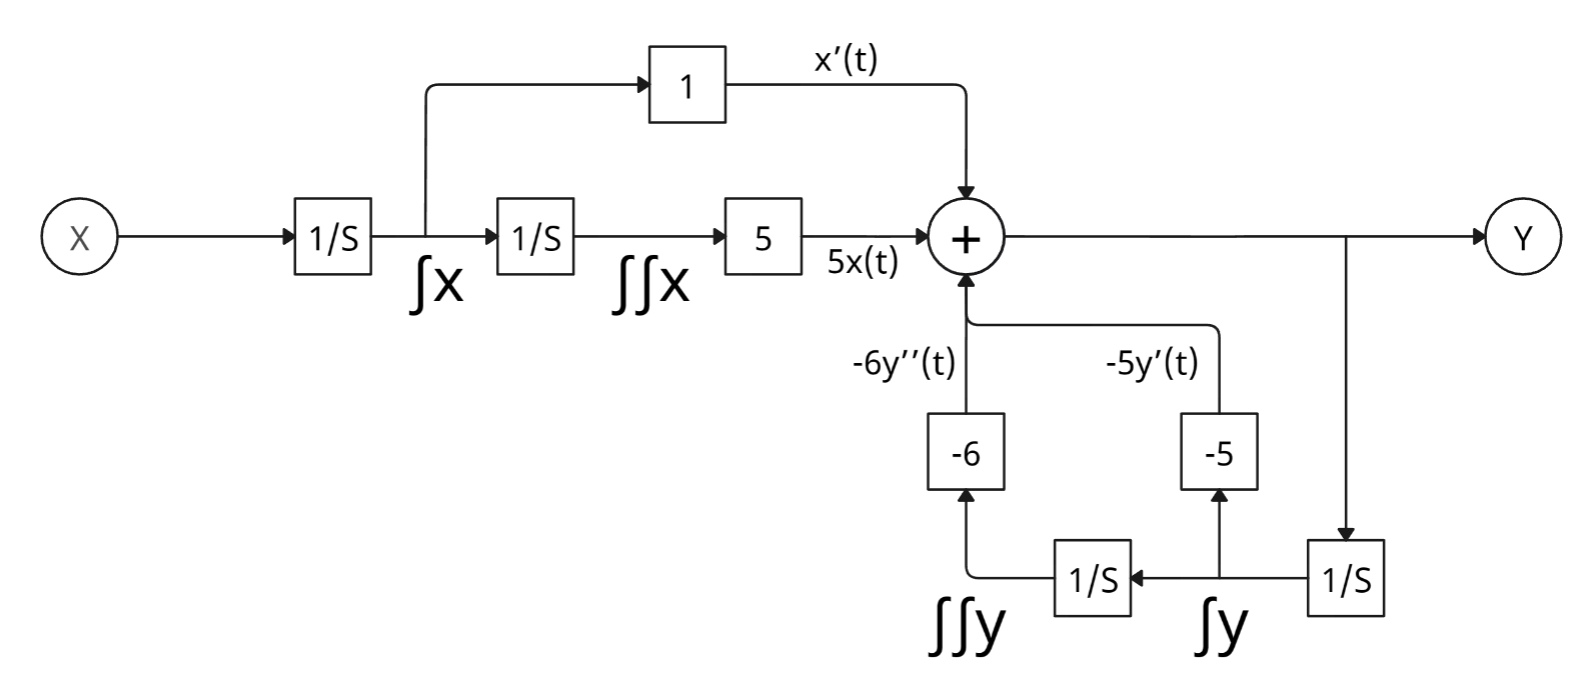
\includegraphics[width=1\textwidth]{p1_block.png}

\subsubsection*{(c)}

The system is stable if all poles of the transfer function have negative real parts. The poles are the roots of:
\begin{equation}
s^2 + 5s + 6 &= (s + 3)(s + 2)
\end{equation}
The poles, \(s = -3\) and \(s = -2\), both have negative real parts. Therefore, the system is stable.

\subsubsection*{(d)}

For a unit step input:
\begin{equation}
x(t) = u(t) \implies X(s) = \frac{1}{s}
\end{equation}
\newline
Using the convolution theorem, the output \( Y(s) \) is:
\begin{equation}
Y(s) = H(s)X(s) = \frac{s + 5}{s^2 + 5s + 6} \times \frac{1}{s}
\end{equation}
\newline
To solve the partial fraction decomposition (PFD) for the expression \(\frac{s+5}{(s+3)(s+2)s}\), we'll decompose it into simpler fractions:

\begin{equation}
\frac{s+5}{(s+3)(s+2)s} = \frac{A}{s+3} + \frac{B}{s+2} + \frac{C}{s}
\end{equation}
\newline
\textbf{To solve for \(A\), \(B\), and \(C\):}
\newline \newline
\textbf{Step 1:}
Multiply each side by the common denominator, which is \((s+3)(s+2)s\):

\begin{equation}
\frac{s + 5}{(s+3)(s+2)s} = \frac{A}{s+3} + \frac{B}{s+2} + \frac{C}{s}
\end{equation}

\begin{equation}
(s+3)(s+2)s \cdot \frac{s + 5}{(s+3)(s+2)s} =  \frac{(s+3)(s+2)s \cdot A}{s+3} + \frac{(s+3)(s+2)s \cdot B}{s+2} + \frac{(s+3)(s+2)s \cdot C}{s}
\end{equation}

\begin{equation}
(s + 5) = (s+2)s A + (s+3)s B + (s+3)(s+2) C
\end{equation}
\newline
\textbf{Step 2:} Plug in values for \(s\) to simplify and solve for \(A\), \(B\), and \(C\):
\newline
\newline
To solve for \(C\), Set \(s = 0\). We choose \(s = 0\) since the A and B terms both cancel out when \(s = 0\).
\newline
From Equation 13:
\begin{align}
(s + 5) &= (s + 2) \cdot s A + (s + 3) \cdot s B + (s+3)(s+2) C \nonumber \\
(0 + 5) &= (0 + 2) \cdot 0 A + (0 + 3) \cdot 0 B + (0+3)(0+2) C \\
5 &= 0 A + 0 B + 6 C \nonumber \\
C &= \frac{5}{6} \nonumber
\end{align}
\newline
To solve for \(B\), Set \(s = -2\). We choose \(s = -2\) since the A and C terms both cancel out when \(s = -2\) due to the \((s+2)\) term.
From Equation 13:
\begin{align}
(s + 5) &= (s + 2) \cdot s A + (s + 3) \cdot s B + (s+3)(s+2) C \nonumber \\
(-2 + 5) &= (-2 + 2) \cdot -2 A + (-2 + 3) \cdot -2 B + (-2+3)(-2+2) C \\
3 &= 0 A + -2 B + 0 C \nonumber \\
B &= -\frac{3}{2} \nonumber
\end{align}
\newline
To solve for \(A\), Set \(s = -3\). We choose \(s = -3\) since the A and C terms both cancel out when \(s = -3\) due to the \((s+3)\) term.
From Equation 13:
\begin{align}
(s + 5) &= (s + 2) \cdot s A + (s + 3) \cdot s B + (s+3)(s+2) C \nonumber \\
(-3 + 5) &= (-3 + 2) \cdot -3 A + (-3 + 3) \cdot -3 B + (-3+3)(-3+2) C \\
2 &= 3 A + 0 B + 0 C \nonumber \\
A &= \frac{2}{3} \nonumber
\end{align}
\newline
Now, we have values for \(A\), \(B\), and \(C\):

\begin{flalign*}
& A = \frac{2}{3} &\\
& B = -\frac{3}{2} &\\
& C = \frac{5}{6} &
\end{flalign*}
\newline
Thus, the partial fraction decomposition is:
\begin{equation}
\frac{s+5}{(s+3)(s+2)s} & = \frac{A}{s+3} + \frac{B}{s+2} + \frac{C}{s} \\
& = \frac{0.667}{s+3} - \frac{1.5}{s+2} + \frac{0.833}{s}
\end{equation}
Using the properties of the inverse Laplace transform, we have:
\begin{equation}
\begin{split}
\mathcal{L}^{-1}\left\{ \frac{s+5}{(s+3)(s+2)s} \right\} & = \mathcal{L}^{-1}\left\{ \frac{0.667}{s+3} \right\} + \mathcal{L}^{-1}\left\{ -\frac{1.5}{s+2} \right\} + \mathcal{L}^{-1}\left\{ \frac{0.833}{s} \right\} \\
& = 0.667e^{-3t} - 1.5e^{-2t} + 0.833
\end{split}
\end{equation}






\newpage

\subsection*{Problem 2 [25 Points]:}
Given the system with the signal flow graph in the following figure,
\newline
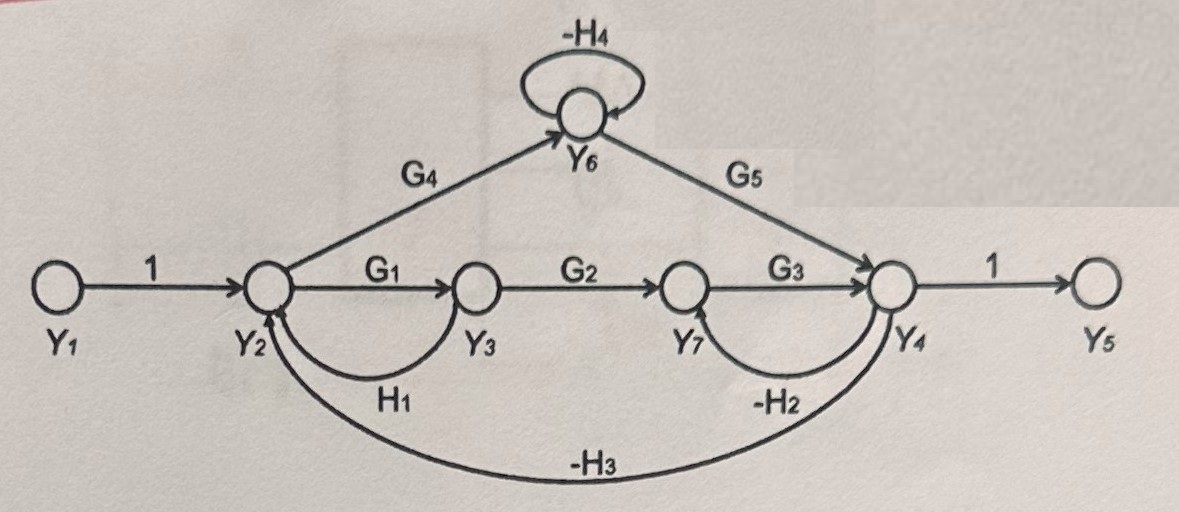
\includegraphics[width=1\textwidth]{p2_SFG.png}
\newline
Compute the transfer function \(\frac{Y_5}{Y_1}\) using Mason's Rule. The intermediate steps must be included.

\subsubsection*{Solution}

Using Mason's Rule for the given signal flow graph:
\subsubsection*{Forward Paths}
\begin{align*}
M_1 & : Y_1 \rightarrow Y_2 \rightarrow Y_3 \rightarrow Y_7 \rightarrow Y_4 \rightarrow Y_5 \\
M_2 & : Y_1 \rightarrow Y_2 \rightarrow Y_6 \rightarrow Y_4 \rightarrow Y_5
\end{align*}
\begin{align*}
\text{Gain of } M_1 & : 1 \times G_1 \times G_2 \times G_3 \times 1 \\
\text{Gain of } M_2 & : 1 \times G_4 \times G_5 \times 1
\end{align*}

\subsubsection*{Loops}
\begin{align*}
L_1 & : Y_2 \rightarrow Y_3 \rightarrow Y_2 \\
L_2 & : Y_7 \rightarrow Y_4 \rightarrow Y_7 \\
L_3 & : Y_2 \rightarrow Y_3 \rightarrow Y_7 \rightarrow Y_4 \rightarrow Y_2 \\
L_4 & : Y_6 \rightarrow Y_6 \\
L_5 & : Y_2 \rightarrow Y_6 \rightarrow Y_4 \rightarrow Y_2
\end{align*}
\begin{align*}
\text{Gain of } L_1 & : G_1 \times H_1 \\
\text{Gain of } L_2 & : -G_3 \times H_2 \\
\text{Gain of } L_3 & : -G_1 \times G_2 \times G_3 \times H_3 \\
\text{Gain of } L_4 & : -H_4 \\
\text{Gain of } L_5 & : -G_4 \times G_5 \times H_3
\end{align*}

\subsubsection*{3-non touching loops}
Only one exists: 
\[ L_4, L_2, L_1 \]
The gain of \( L_{421} \) is:
\[ -H_4 \times (-G_3 \times H_2 \times G_1 \times H_1) \]

\subsubsection*{2-non touching loops}
\begin{align*}
\text{Gain of } L_{21} & : -G_3 \times H_2 \times G_1 \times H_1 \\
\text{Gain of } L_{41} & : -H_4 \times G_1 \times H_1 \\
\text{Gain of } L_{42} & : -H_4 \times (-G_3 \times H_2) \\
\text{Gain of } L_{43} & : -H_4 \times (-G_1 \times G_2 \times G_3 \times H_3 \\
\end{align*}
\subsubsection*{Calculating \( \Delta \)}
\begin{align*}
\Delta & = 1 - (L_1 + L_2 + L_3 + L_4 + L_5) + (L_{21} + L_{42} + L_{41} + L_{43}) - L_{421} \\
& = 1 - (G_1 \times H_1 - G_3 \times H_2 - G_1 \times G_2 \times G_3 \times H_3 - H_4) \\
& + (-G_3 \times H_2 \times G_1 \times H_1 - H_4 \times G_1 \times H_1 + H_4 \times G_3 \times H_2 + H_4 \times G_1 \times G_2 \times G_3 \times H_3) \\
& + H_4 \times G_3 \times H_2 \times G_1 \times H_1
\end{align*}
\subsubsection*{Calculating Gain}
\begin{align*}
\text{Because } M_2 \text{ touches all loops, } \Delta_2 & = 1; \\
\text{Because } M_1 \text{ touches all but } L_4, \Delta_1 & = 1 - L_4 = 1 + H_4
\end{align*}

\begin{align*}
M = \frac{Y_5}{Y_1} & = \frac{M_1 \Delta_1 + M_2 \Delta_2}{\Delta} \\
& = \frac{(1 - L_4) \times 1 \times G_1 \times G_2 \times G_3 \times 1 + 1 \times 1 \times G_4 \times G_5 \times 1}{\Delta}
\end{align*}

\end{document}
